\documentclass[10pt]{report}

\usepackage{amsmath}
\usepackage{amssymb}
\usepackage{array}
\usepackage{tabu}
\usepackage{lmodern}
\usepackage{graphicx}
\usepackage[space]{grffile}
\usepackage{subfigure}
\usepackage{longtable}

\begin{document}
	Optimization problem for estimation of kinetic parameters from noisy experimental data. The noisy data is generated through the use of additive noise in flux equations that use a known kinetic model to predict the responses of a metabolic network to different perturbations.\\
	\begin{equation}
	v^* = g(x,p) + {\cal{N}}(0,1)
	\end{equation}
	where ${\cal{N}}(0,1)$ is Gaussian noise with zero mean and a standard deviation of 1.
	\begin{equation}\label{eq:ode1}
	\frac{d}{dt}pep=v_1-v_2-v_4
	\end{equation}
	\begin{equation}\label{eq:ode2}
	\frac{d}{dt}fdp=v_2-v_3
	\end{equation}
	\begin{equation}\label{eq:ode3}
	\frac{d}{dt}E=v_{e,max}\left(\frac{1}{1+\left(\frac{fdp}{K_{e}^{fdp}}\right)^{n_e}}\right) - d E
	\end{equation}
	The kinetic expressions for fluxes $v_1$ through $v_4$ are given below. The consumption of acetate through $v_1$ and conversion of \textit{pep} through $v_2$ are expressed in Equations (\ref{eq:flux1}) and (\ref{eq:flux2}) respectively using Michaelis-Menten kinetics. The acetate flux through $v_1$ is also governed by the quantity of available enzyme E. 
	\begin{equation}\label{eq:flux1}
	v_1 = k_{1}^{cat}E\frac{acetate}{acetate+K_{1}^{acetate}}
	\end{equation}	
	\begin{equation}\label{eq:flux2}
	v_2 = V_{2}^{max}\frac{pep}{pep+K_{2}^{pep}}
	\end{equation}
	\begin{equation}\label{eq:flux3}
	v_3 = V_{3}^{max}\frac{\tilde{fdp}\left(1+\tilde{fdp}\right)^3}{\left(1+\tilde{fdp}\right)^4+L_3\left(1+\frac{pep}{K_{3}^{pep}}\right)^{-4}}
	\end{equation}
	The allosterically regulated flux $v_3$ for the consumption of \textit{fdp} is expressed in Equation (\ref{eq:flux3}) using the Monod-Wyman-Changeux (MWC) model for allosterically regulated enzymes, where $\tilde{fdp}$ refers to the ratio of \textit{fdp} with respect to its allosteric binding constant $K_{3}^{fdp}$. The added flux $v_4$ for the export of \textit{pep} is expressed as a linear equation dependent on $pep$ in Equation (\ref{eq:flux4}).
	\begin{equation}\label{eq:flux4}
	v_4 = k_{4}^{cat}.pep
	\end{equation}
	
	We denote the known noisy flux and concentration information with the superscript $^*$. Accordingly, fluxes $v^*$ and concentrations $x^*$ are the noisy information that will be used for estimation. Fluxes ($v$) and concentrations ($x$) that predicted by the model (without noise) are denoted without the superscript.
	
	The optimization formulation to estimate fluxes given below is based on the minimization of the tolerance for the L2-norm of the difference between the model predicted flux and the noisy flux. 
	\begin{center}
		\begin{subequations}\label{eq:noisyopt}
			\begin{align}
			\underset{x,p,e}{\mathrm{min}} & \text{      }e\\
			\mathrm{st} & \text{      }|v-v^*| \le \varepsilon\\
			& \text{      }|x-x^*| \le \varepsilon\\
			& \text{      }Sv = 0\\
			& \text{      }v = f(x,p) + e\\
			& \text{      }x_{min}\le x \le x_{max}\\
			& \text{      }p_{min} \le p \le p_{max}\\	
			& \text{      }e_{min} \le e \le e_{max}						
			\end{align}
		\end{subequations}		
	\end{center}

	In Equation (\ref{eq:noisyopt}) above, $\varepsilon$ is the absolute tolerance between the predicted and the measured quantities. The relationship between the predicted and the measured quantities are given by the nonlinear constraints in Equations (\ref{eq:noisyopt}b) and (\ref{eq:noisyopt}c). The stoichiometric constraints for steady state are given by Equation (\ref{eq:noisyopt}d), and Equation (\ref{eq:noisyopt}e) specifies the kinetic rate laws for the predicted fluxes as a function of the concentrations ($x$) and the parameters ($p$). Equations (\ref{eq:noisyopt}f) and (\ref{eq:noisyopt}g) are the bounds for the concentrations and parameters that are to be estimated by the optimization problem. The above optimization problem is to be solved for fixed values of $\varepsilon \in \{\text{.01, .05, .1}\}$.	
	
	\paragraph{Changes in problem formulation due to feasibility issues:}
	Since the above problem (Equation \ref{eq:noisyopt}) does not result in feasible global optimal solutions (using SCIP), the constraints are relaxed and the feasible problem is presented below.
	
	\begin{center}
		\begin{subequations}\label{eq:optmod}
			\begin{align}
			\underset{x,p_i,e_i}{\mathrm{min}} & \text{      }e_i\\
			\mathrm{st} & \text{      }|v_i-v^*| \le 0.2\\
			& \text{      }|x-x^*| \le 0.3\\
			& \text{      }|Sv| \le 1\text{x}10^{-8}\\
			& \text{      }v_i = f(x,p_i) + e\\
			& \text{      }v_{j\not= i} = f(x,p_{j\not=i})\\
			& \text{      }x_{min}\le x \le x_{max}\\
			& \text{      }p_{i,min} \le p_i \le p_{i,max}\\
			& \text{      }e_{i,min} \le e_i \le e_{i,max}					
			\end{align}
		\end{subequations}		
	\end{center}
	
	In Equation (\ref{eq:optmod}) above, the index $i$ represents the flux whose parameters are being optimized and index $j$ represents all other fluxes whose parameters are held constant. 
	
	The steady state constraint has been relaxed (from a equality constraint to an inequality constraint) along with permitting the concentrations and the estimated fluxes to deviate significantly from their experimentally observed values (~20 - 30\%). 
	
	The bounds for the flux noise were set at (0,20) in the above problem.
	
	\paragraph{Suggested modifications to address infeasibility (July 4)}
	After discussion with Prof. M, the following changes were made to the problem formulation:
	\begin{itemize}
		\item Experimental fluxes may/may not be at steady state. Accordingly, using the steady state constraint in the above formulation can render the optimization problem infeasible. Suggestion is to remove this constraint(s).
		\item Include the norm minimization constraint as an objective.
		\item Add the noise in fluxes and concentrations as part of the bound constraint.
		\begin{center}
			\begin{subequations}
				\begin{align}
				\underset{x,p_j}{\mathrm{min}} & \text{      }\left\Vert v_i-v^*\right\Vert &  i\in\mathcal{R}^n,\text{  }j\in\mathcal{R}^l\\
				\mathrm{st}& \text{      }v_i = f(x,p_j)\\
				& \text{      }x_{min}(1-\epsilon)\le x \le x_{max}(1+\epsilon)\\
				%& \text{      }v_{min}(1-\epsilon)\le v \le v_{max}(1+\epsilon)\\
				& \text{      }p_{j,min} \le p_j \le p_{j,max}
				\end{align}
			\end{subequations}
		\end{center}
	\item The noise $\epsilon$ is fixed at 5\% or 10\% to signify experimental noise.
	\end{itemize}

	\paragraph{More changes to address nonlinearity due to division(July 13)}
	Prof. M suggested changing the nonlinear formulation of the flux equations into just a bilinear form by removing the denominator and formulating it as nonlinear algebraic equation.
	\begin{center}
		\begin{subequations}
			\begin{align}
			\underset{x,p_j,v_i}{\mathrm{min}} & \text{      }\left\Vert v_i-v^*\right\Vert &  i\in\mathcal{R}^n,\text{  }j\in\mathcal{R}^l\\
			\mathrm{st}& \text{      }N(x,p_j) - v_iD(x,p_j) = 0\\
			& \text{      }x_{min}(1-\epsilon)\le x \le x_{max}(1+\epsilon)\\			
			& \text{      }p_{j,min} \le p_j \le p_{j,max}\\
			& \text{      }v_{i,min}(1-\epsilon)\le v_i \le v_{i,max}(1+\epsilon)
			\end{align}
		\end{subequations}
	\end{center}

	\begin{itemize}
		\item Also, the initial noise added to the steady state solutions was reduced from 50\% to 5\% or 10\%.
		\item $\epsilon$ is fixed at 50\%.
		\item Solution is obtained using multisolve with IPOPT instead of aiming to obtain a global solution with SCIP.
		\item Using approximately 14 million points for the second phase of multistart in OPTI
	\end{itemize}

\paragraph{Changes in formulation}
This formulation assumes that the concentrations and the fluxes corresponding to each perturbation are variables in the optimization problem formulated to estimate kinetic parameters.

Let $\mathbf{x}\in\mathbb{R}^m$, $\mathbf{p}\in\mathbb{R}^l$ and $\mathbf{v}\in\mathbb{R}$ be the vector of concentrations, parameters and fluxes respectively. If the number of perturbations used for parameter estimation is in $\mathbb{R}^p$, then the vector of concentrations, fluxes and parameters that need to be estimated in the optimization problem changes to $\mathbf{x}\in\mathbb{R}^{mp}, \mathbf{v}\in\mathbb{R}^{p}$ and $\mathbf{p}\in\mathbb{R}^{l}$ respectively. 

Let $i\in\mathbb{R}^{mp}$, $j\in\mathbb{R}^{p}$ and $k\in\mathbb{R}^{l}$ represent the indices for concentrations, fluxes and parameters respectively.

\begin{center}
	\begin{subequations}
		\begin{align}
		\underset{\mathbf{x},\mathbf{p},\mathbf{v}}{\mathrm{min}} & \text{      }\left\Vert \mathbf{v}-\mathbf{v}^*\right\Vert\\
		\mathrm{st}& \text{      }N(\mathbf{x},\mathbf{p}) - v_jD(\mathbf{x},\mathbf{p}) = 0 & \text{  }\forall & \text{ }j\in\mathbb{R}^p\\
		& \text{      }x^*_i(1-\epsilon)\le x_i \le x^*_i(1+\epsilon) & \text{  }\forall & \text{ }i\in\mathbb{R}^{mp}\\	
		& \text{      }v^*_j(1-\epsilon)\le v_j \le v^*_j(1+\epsilon) & \text{  }\forall & \text{ }j\in\mathbb{R}^{p}\\		
		& \text{      }\mathbf{p}_{min} \le \mathbf{p} \le \mathbf{p}_{max}
		\end{align}
	\end{subequations}
\end{center}

	\paragraph{Results:}
	These are the results from the parameter estimation algorithm that we have been running. I have tried estimating parameters for the Kotte model by using noisy perturbation data.
	
	\begin{figure}[!h]%figure1
		\centering{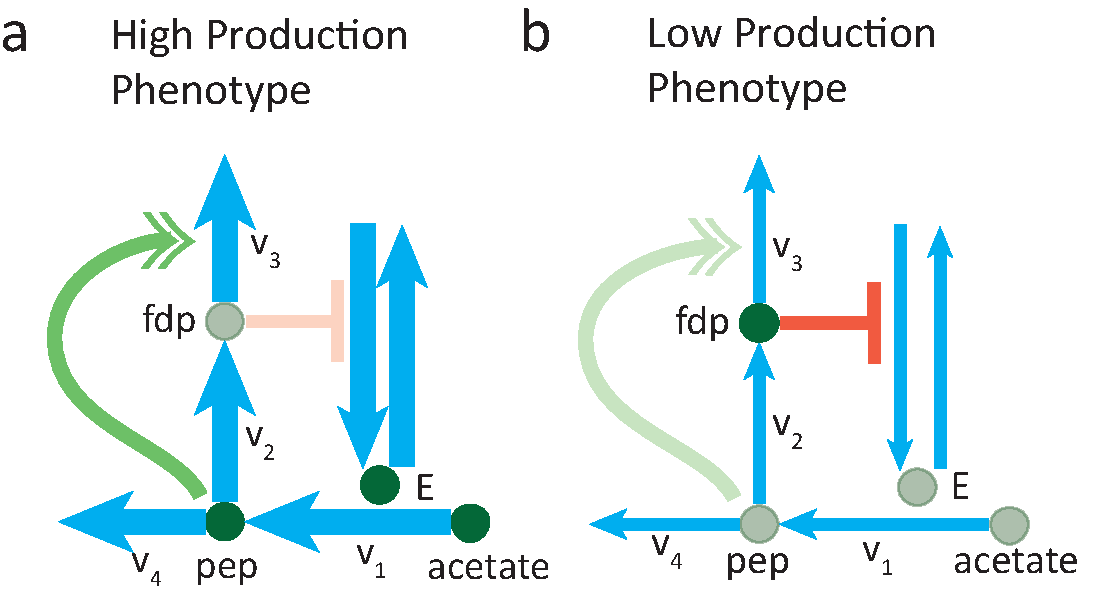
\includegraphics[width=0.6\textwidth,height=1.0\textheight,keepaspectratio]{figures/figure1_phenotypes.pdf}}
		\caption{The two stable phenotypes for acetate consumption through the gluconeogenic model. a) The high production phenotype which has a high flux throughout the network as a result of a high \textit{pep} concentration that reduces the inhibition on acetate uptake and b) The low production phenotype that is characterized by a relatively low \textit{pep} concentration and consequently increased inhibition on the acetate uptake as a result of a smaller \textit{fdp}.}\label{fig:fig1}
	\end{figure}

	\begin{table}[!tbhp]
		\caption{Table showing the perturbed values of all fluxes used for parameter estimation.}
		\begin{center}				
			\begin{tabular}{ccc}
				Designation & Perturbed Fluxes & Perturbed Values\\
				\hline
				P1 & $v_1$ & 2\\
				P2 & $v_2$ & 0.2\\
				P3 & $v_3$ & 0.5
			\end{tabular}
		\end{center}	
	\label{tab:pval}
	\end{table}
	
	\paragraph{Estimation for $v_1$}: The steady state data from the above perturbations in Table \ref{tab:pval} were used to estimate the value of the parameters $k_1^{cat}$ and $K_1^{acetate}$ for flux $v_1$.
	
	The comparison of the estimated and the experimental (noisy model generated) data are shown below. Notice that the model estimates do not match well with the noisy data for perturbation P1 (Table \ref{tab:pval}). This is the observed case for all other parameter estimations. This could be due to the effect of perturbation to the acetate uptake flux ($v_1$) on the steady states of the system. (Note that a higher acetate uptake flux lets the system reach the higher steady state).
	
	\begin{figure}[!tbhp]
		\centering{\includegraphics[width=1.0\textwidth,height=1.0\textheight,keepaspectratio]{C:/Users/shyam/Documents/Courses/CHE1125Project/Results/estimation/est_flux1/est_flux1_conc_Jul20}}
		\caption{Plot comparing noisy model generated steady state metabolite concentrations with model estimates obtained using an optimized model for $v_1$. pep, fdp and enzyme E (Top to bottom)}
	\end{figure}
	\begin{figure}[!tbhp]
		\centering{\includegraphics[width=1.0\textwidth,height=1.0\textheight,keepaspectratio]{C:/Users/shyam/Documents/Courses/CHE1125Project/Results/estimation/est_flux1/est_flux1_flux_Jul20}}
		\caption{plot comparing noisy model generated steady state fluxes with model estimates obtained using an optimized model for $v_1$.}
	\end{figure}
	\clearpage

	\paragraph{Estimation for $v_2$}: The steady state data from the above perturbations in Table \ref{tab:pval} were used to estimate the value of the parameters $V_2^{max}$ and $K_2^{pep}$ for flux $v_2$.
		
	\begin{figure}[!tbhp]
		\centering{\includegraphics[width=1.0\textwidth,height=1.0\textheight,keepaspectratio]{C:/Users/shyam/Documents/Courses/CHE1125Project/Results/estimation/est_flux2/est_flux2_conc_Jul20}}
		\caption{Plot comparing noisy model generated steady state metabolite concentrations with model estimates obtained using an optimized model for $v_2$. pep, fdp and enzyme E (Top to bottom)}
	\end{figure}
	\begin{figure}[!tbhp]
		\centering{\includegraphics[width=1.0\textwidth,height=1.0\textheight,keepaspectratio]{C:/Users/shyam/Documents/Courses/CHE1125Project/Results/estimation/est_flux2/est_flux2_flux_Jul20}}
		\caption{plot comparing noisy model generated steady state fluxes with model estimates obtained using an optimized model for $v_2$.}
	\end{figure}

	The estimation of parameter for flux $v_2$ also runs into the same issues mentioned above for flux $v_1$.	
	
	\paragraph{Estimation for $v_3$}: The steady state data from the above perturbations in Table \ref{tab:pval} were used to estimate the value of the parameters $V_3^{max}$, $K_3^{fdp}$ and $K_3^{pep}$ for flux $v_2$. 
	
	The optimization cannot find an optimal solution for this problem. The optimization problem using IPOPT with the OPTI Toolbox  ends with a cannot find an optimal solution error despite increasing the number of multistart points considerably.
	
	\begin{itemize}
		\item Noise to original steady state was 5\%.
		\item Bounds for both fluxes and concentrations in the aforementioned formulation were fixed at 50\%.
	\end{itemize} 

	
\end{document}

